\begingroup

\let\clearpage\relax
\chapter{Indexability}
\label{chp:apx_indexability}

\subsection{Unichain property}

\begin{lem}
\label{lem:invertible}
Given a two-action MDP $\langle [n], \{0,1\}, r, P\rangle$, let $\mP^\pi$ be the transition matrix under a Bellman optimal policy $\pi$.
Policy $\pi$ is \emph{unichain} if and only if the matrix
\begin{align*}
    \mA^{\pi}
        = \left[\begin{array}{ccccc}
                1 & - P_{12}^{\pi} & \dots & -P_{1n}^{\pi}\\
                1 & 1-P_{22}^{\pi} & \dots & -P_{2n}^{\pi}\\
                \vdots\\
                1 &  -P_{n2}^{\pi} & \dots &1-P_{nn}^{\pi}
    \end{array}\right]
\end{align*}
is invertible.
\end{lem}
\begin{proof}
    $\mA^\pi$ is not invertible if there exists a column vector $\vu\neq\vzero$ such that $\vu^\top \mA^\pi=\vzero$.
    We prove that such $\vu$ does not exist when policy $\pi$ is unichain.
    Let $\vu\in\real^n$ be an arbitrary vector such that $\vu^\top \mA^\pi=\vzero$.
    Then, we have
    \begin{align*}
        \begin{cases}
            \sum_{i=1}^{n}u_i &= 0 \\
            u_i-\sum_{j=1}^{n}u_jP_{ji}^\pi &= 0, \text{ for } 2\le i\le n
        \end{cases}
    \end{align*}
    Combining the above equation with $\sum_j P^\pi_{ji}=1$, we get:
    \begin{align*}
        u_1 &= -\sum_{i=2}^n u_i
        =-\sum_{i=2}^n\sum_{j=1}^n u_j P^\pi_{ji}
        =-\sum_{j=1}^n u_j (1-P^\pi_{j1})
        = \sum_{j=1}^n u_j P^\pi_{j1},
    \end{align*}
    where we used that $\sum_{i=1}^{n}u_i=0$ to obtain the last equality.  
    This shows that 
    \begin{align*}
        \begin{cases}
            \sum_{i=1}^{n}u_i &= 0 \\
            \vu^\top\mP^\pi &=\vu^T
        \end{cases}
    \end{align*}
    The set of vector $\vu$ such that $\vu^\top\mP^\pi$ is a vector space. It is of dimension $1$ if and only if $\pi$ is unichain, in which case the vector $\vu$ verifying $\vu^\top\mP^\pi=\vu^\top$ are multiples of a stationary distribution under policy $\pi$ \cite{puterman2014markov}. Thus, if the policy $\pi$ induces a unichain Markov chain, then $\sum_{i=1}^{n}u_i = 0$ implies $\vu = \vzero$. If policy $\pi$ is not unichain, there exists $\vu\ne\vzero$ such that $\sum_{i=1}^{n}u_i = 0$.
%    However, such vector is a distribution, \emph{i.e.}, $\sum_{i=1}^{n}u_i=1$.
\end{proof}

\section{Implementations}
\label{apx:implementation}

\subsection{Arithmetic complexity of Subroutine~\ref{algo:update_X} and memory usage}

Recall that in Subroutine~\ref{algo:update_X}, we compute the values $X^{\ell}_{ij}$ by doing the update (for all iteration $k$, for all $\ell=1$ to $k$ and for all $i\in[n]$ or all $i\in\pi^{\ell+1}$ if we do not test indexability):
\begin{align}
    \label{eq:apx_update}
    X_{i\sigma^{k}}^{\ell+1} = X_{i\sigma^{k}}^{\ell} -\displaystyle\frac{X^{\ell}_{i\sigma^{\ell}}}{1+X^{\ell}_{\sigma^{\ell}\sigma^{\ell}}}X^{\ell}_{\sigma^{\ell}\sigma^{k}}
\end{align}

If we test indexability, there are $\sum_{k=1}^nk n = n^3/2+O(n^2)$ such updates. If we do not test indexability, there are $\sum_{k=1}^n \sum_{\ell=1}^k (n-\ell) = n^3/3 + O(n^2)$ such updates.  Below, we show each update of Equation~\eqref{eq:apx_update} can be done in two arithmetic operations (one addition and one multiplication), which leads to the complexity of $n^3+O(n^2)$ (or $(2/3)n^3+O(n^2)$) arithmetic operations for the computation of all the needed $X^k_{ij}$.  We also show how to reduce the memory size to $O(n^2)$.

Let $W_{i\ell} := X^\ell_{i \sigma^\ell}/(1+X^\ell_{\sigma^\ell\sigma^\ell})$ and $V_i :=X^\ell_{i\sigma^k}$. Using this, Equation~\eqref{eq:apx_update} can be rewritten as: 
\begin{align}
    \label{eq:apx_update_V}
    V_{i} = V_{i} - W_{i\ell} V_{\sigma^{\ell}}.
\end{align}

This results in the following loop at iteration $k$:
\begin{itemize}
    \item Initialize $V_{i}$ from $X^1_{i\sigma^k}$. 
    \item For all $\ell\in\{1,\dots, k-1\}$, and all $i\in[n]$ (or $i\in\pi^{\ell+1}$), apply \eqref{eq:apx_update_V}. 
    \item Compute $W_{ik}= V_{i}/(1+V_{\sigma^k})$
\end{itemize}
Note that the value of $\mV$ is not necessary for iteration $k$ (only the values of $W_{i\ell}$ are needed). This shows that the algorithm can be implemented with a memory $O(n^2)$.% Moreover, each update of \eqref{eq:apx_update} can be implemented by $2$ arithmetic operations (one multiplication and one subtraction). 

\subsection{Speedup when not checking the indexability: First found go last} 

When the indexability is not tested, the update \eqref{eq:apx_update_V} is computed for all $i\in\pi^{\ell+1}$. This creates inefficiencies (due to  inefficient cache usage) because the elements $V_{i}$ are not accessed sequentially.

To speedup the memory accesses, our solution is to sort the items during the execution of the algorithm. At iteration $k$, the algorithm computes $\sigma^{k}$. When this is done, our implementation switches all quantities in positions $\sigma^{k}$ and $n-k+1$. These quantities are $\delta, y, z, \mW$ and $\mX$. For instance, once $\sigma^1$ is found, we know that the state at position $n$ is state $n$ and we do the following switches:
\begin{align*}
    \delta_{\sigma^1}, \delta_{n} &\rightarrow \delta_{n}, \delta_{\sigma^1} \\
    y^1_{\sigma^1}, y^1_{n} &\rightarrow y^1_{n}, y^1_{\sigma^1} \\
    z^1_{\sigma^1}, z^1_{n} &\rightarrow z^1_{n}, z^1_{\sigma^1} \\
    \mW_{\sigma^1 :}, \mW_{n :} &\rightarrow \mW_{n:}, \mW_{\sigma^1:} \\
    \text{ and } \mX_{\sigma^1 :}, \mX_{n :} &\rightarrow \mX_{n :}, \mX_{\sigma^1 :}.
\end{align*}

To do so, we need an array to store all states such that at iteration $k$, the first $n-k$ states of the array are the active states. We will need to track the position of each state in such array.

\section{Analysis of the experimental time to solve a linear system}
\label{apx:inversion}

In this section, we report in Figure~\ref{fig:benchmark_inverse} the time taken by the default implementation to solve a linear system of the form $\mA\mX=\mB$ where $\mA$ and $\mB$ are two square matrices. To obtain this figure, we generated random (full) matrices where each entry is between $0$ and $1$ and use the function  \texttt{scipy.linalg.solve} from the library \texttt{scipy}. The reported numbers suggest that the complexity of the solver is closer to $O(n^{2.8})$ than to $O(n^3)$, although we agree that the difference between the $O(n^{2.8})$ and the $O(n^3)$ curves is small. Note that this is in accordance with the papers \cite{huang2016strassen,huang2018practical} that claim that the fastest implementations of matrix multiplication and inversion are based on Strassen's algorithm and should therefore be in $O(n^{2.8})$. 

\begin{figure}[ht]
    \centering
    \begin{tabular}{cc}
        \begin{minipage}{0.5\linewidth}
            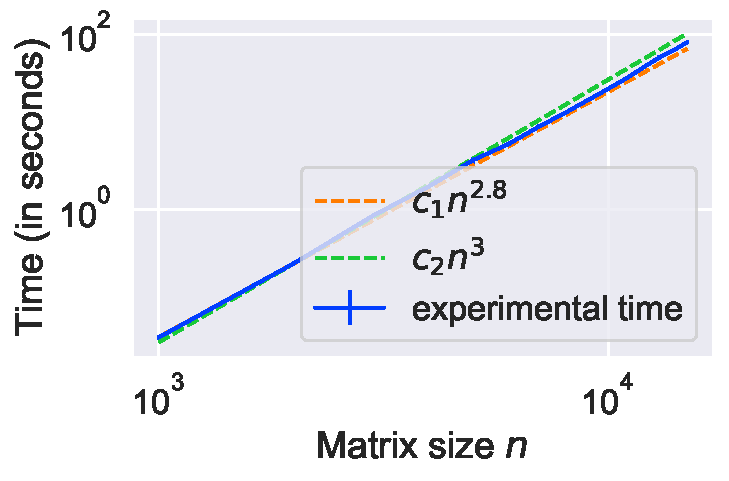
\includegraphics[width=\linewidth]{execution_time_solve}
        \end{minipage}
        %\includegraphics[width=0.4\linewidth]{execution_time_inversion}
        %&\includegraphics[width=0.4\linewidth]{execution_time_multiplication}\\
        &\begin{minipage}{0.45\linewidth}
            \begin{tabular}{|c|c|}
                \hline
                $n$ & Time (in second)\\\hline
                1000 & $ 0.03\pm0.02$ \\
                2000 & $ 0.24\pm0.01$ \\
                4000 & $ 1.83\pm0.05$ \\
                5000 & $ 3.6\pm0.3$ \\
                7000 & $ 8.7\pm0.5$ \\
                10000 & $23.7\pm0.6$ \\
                13000 & $54.0\pm2.5$ \\
                15000 & $80.8\pm1.8$ \\                
                \hline
            \end{tabular}
        \end{minipage}
    \end{tabular}
    \caption{Time taken of the default implementations \texttt{scipy.linalg.solve} of scipy to solve a linear system $\mA\mX=\mB$ where $\mA$ and $\mB$ are two square $n\times n$ matrices.}
    \label{fig:benchmark_inverse}
\end{figure}

%%%%%%%%%%%%%%%%%%%%%%%%%%%%%%%%%%%%%%%%%%%%%%%%%%%%%%%%%%%%%%%%%%%%%%%%%%%%%%%%%%%%%%%%%%%%%%%%%%%
%%%%%%%%%%%%%%%%%%%%%%%%%%%%%%%%%%%%%%%%%%%%%%%%%%%%%%%%%%%%%%%%%%%%%%%%%%%%%%%%%%%%%%%%%%%%%%%%%%%
\section{Detailed comparison with \texorpdfstring{\cite{akbarzadeh2020conditions} and \cite{nino2020fast}}{Akbarzadeh et al. 2020 and Nino Mora 2020.}}
\label{apx:comparison}

In this section, we compare our algorithm with two main related works for finite-state restless bandits problem.

\subsection{Comparison with \texorpdfstring{\cite{akbarzadeh2020conditions}}{Akbarzadeh2020 et al. 2022}}
The paper presents an  algorithm that computes Whittle indices  in $O(n^3)$ (no explicit constant before $n^3$ is given) for all indexable problems. Despite following a different approach, our algorithm for computing Whittle index can be viewed as a refinement of this work. Let us recall once again that our approach also allows one to check the indexability of general restless bandits.

In the following, we show how we can refine the work of \cite{akbarzadeh2020conditions} to obtain an algorithm that is exactly the same as ours.
%Let $\Phi^\pi$ be a square matrix and $D^{\pi}$ and $N^{\pi}$ be two vectors defined as in \cite{akbarzadeh2020conditions},
Let $D^{\pi}$ and $N^{\pi}$ be two vectors defined as in \cite{akbarzadeh2020conditions} (we use the same notation,  $D^{\pi}$ and $N^{\pi}$, as the cited paper),
\begin{align*}
    %\Phi^\pi = (I-\beta P^\pi)^{-1}, \quad
    D^{\pi} =(1-\beta)(\mI-\beta \mP^\pi)^{-1}\vr^{\pi}, \quad\text{and}\quad
    N^{\pi} =(1-\beta)(\mI-\beta \mP^\pi)^{-1}\vpi.
\end{align*}
Then, we have $D^{\pi} -\widx N^{\pi}=(1-\beta)\vu^{\pi}(\widx)$ where $\vu^{\pi}(\widx)$ is defined as in \eqref{eq:h is linear discounted}. In our proposition, at each iteration $k$, we compute $\mu_i^k$ by Line~\ref{algo2:muki}. Instead, it is defined in \cite{akbarzadeh2020conditions} by two steps:
\begin{enumerate}
\item for all state $j\in[n]$ such that $N_j^{\pi^k\setminus\{i\}}{\neq} N_j^{\pi^k}$, one needs to compute $\mu^k_{ij}{=}\displaystyle\frac{D_j^{\pi^k\setminus\{i\}} -D_j^{\pi^k}}{ N_j^{\pi^k\setminus\{i\}} -N_j^{\pi^k}}$ 
\item \label{it:mu^k_i*} compute $\mu^k_i=\displaystyle\argmin_{j\in[n]:N_j^{\pi^k\setminus\{i\}}\neq N_j^{\pi^k}} \mu^k_{ij}$.
\end{enumerate}
From \cite[Theorem 2]{akbarzadeh2020conditions}, in an indexable problem, for state $\sigma^k$, there exists a state $j\in[n]$ such that $N_j^{\pi^k\setminus\{\sigma^k\}}\neq N_j^{\pi^k}$. Now, suppose that for any active state $i\in\pi^k$, there exists $j\in[n]$ such that $N_j^{\pi^k\setminus\{i\}}\neq N_j^{\pi^k}$. Using the Sherman-Morrison formula, we have\footnote{the expression of $D^{\pi\setminus\{i\}}$ and $N^{\pi\setminus\{i\}}$ given by Equation~$(18)$ in \cite{akbarzadeh2020conditions} are erroneous.}
\begin{align*}
    &D^{\pi^k\setminus\{i\}} -D^{\pi^k} = -\frac{(1-\beta)\delta_i +\tilde{\mDelta}_iD^{\pi^k}}{1+\tilde{\mDelta}_i[(\mI-\beta \mP^{\pi^k})^{-1}]_{: i}}[(\mI-\beta \mP^{\pi^k})^{-1}]_{: i}, \\
    &\quad \text{and}\quad N^{\pi^k\setminus\{i\}} -N^{\pi^k} = -\frac{(1-\beta) +\tilde{\mDelta}_iN^{\pi^k}}{1+\tilde{\mDelta}_i[(\mI-\beta \mP^{\pi^k})^{-1}]_{: i}}[(\mI-\beta \mP^{\pi^k})^{-1}]_{: i}.
\end{align*}
Then, for any $j\in[n]$ such that $N_j^{\pi^k\setminus\{i\}}\neq N_j^{\pi^k}$, $\mu^k_{ij}=\displaystyle\frac{(1-\beta)\delta_i +\tilde{\mDelta}_iD^{\pi^k}}{(1-\beta) +\tilde{\mDelta}_iN^{\pi^k}}$ which does not depend on $j$.
Then, we simply have ${\mu^k_i=\displaystyle\frac{(1-\beta)\delta_i +\tilde{\mDelta}_iD^{\pi^k}}{(1-\beta) +\tilde{\mDelta}_iN^{\pi^k}}}$. %=\frac{\tilde{\Delta}_i((1-\beta)\vu^{\pi^k}(\mu^k_i)+\mu_i^kN^{\pi^k})}{\tilde{\Delta}_iN^{\pi^k}}$.
Also, we have 
\begin{align*}
    \tilde{\mDelta}_iN^{\pi^k}&=(1-\beta)\tilde{\mDelta}_i(\mI-\beta \mP^{\pi^k})^{-1}\vpi^k=-(1-\beta)y^k_i \quad\text{and}\\
    \tilde{\mDelta}_iD^{\pi^k}&={(1-\beta)\tilde{\mDelta}_i\vu^{\pi^k}(\mu^{k-1}_{\min}) +\mu^{k-1}_{\min}\tilde{\mDelta}_i N^{\pi^k}} =(1-\beta)z^{k-1}_i -(1-\beta)\mu^{k-1}_{\min}y^k_i.
\end{align*}
So, replacing these terms in $\mu^k_i$, we get the formula in Equation~\eqref{eq:mu^k_i_from_y} of our work.

Note that the algorithm of \cite{akbarzadeh2020conditions} was only developed for the discounted case.  Our approach for the time-average reward case is different because we use the active advantage function defined in \eqref{eq:advantage} instead of working with the expected discounted total reward $D^{\pi^k}$ and total number of activations $N^{\pi^k}$ under policy $\pi^k$. 
Note that the counterpart of $D^{\pi^k}$ in undiscounted MDP is the average reward $g^{\pi^k}$ and as we have seen in Appendix~\ref{apx:discussion_index}, utilizing average reward optimality is not rich enough for undiscounted MDPs with transient states.
In addition, our code is also optimized to avoid unnecessary computation and to reduce memory usage. Finally, the way we do the update of our matrix $\mX$ makes it possible to obtain a subcubic algorithm whereas their approach does not (see also below).

\subsection{Comparison with the algorithm of \texorpdfstring{\cite{nino2020fast}}{Nino Mora 2020}}
The algorithm \cite{nino2020fast} has the best complexity up to date for discounted restless bandit. There is a square matrix $\mA$ that plays a similar role as the square matrix $\mX$ in our proposed algorithm. The most costly operations in the algorithm of \cite{nino2020fast} is to update their matrix $\mA$ at each iteration and it is done by Equation~\eqref{eq:update_X_naif} that we recall here (using the same notation $\mA$ as the cited paper):
\begin{align}
    \label{eq:15}
    \text{for } i,j\in\pi^k,\ \mA^{k+1}_{ij}= \mA^{k}_{ij} -\frac{\mA^{k}_{i\sigma^k}}{\mA^{k}_{\sigma^k\sigma^k}}\mA^{k}_{\sigma^kj}.
\end{align}
This incurs a total complexity of $(2/3)n^3+O(n^2)$ arithmetic operations.
As mentioned in Section~\ref{ssec:two_third_algo}, if we updated $\mX^{k+1}$ as given by \eqref{eq:update_X_naif}, our algorithm would also have a $(2/3)n^3+O(n^2)$ complexity but this version of update cannot be optimized by using  fast matrix multiplication.

\subsection{Their approach cannot be directly transformed into a subcubic algorithm}
\label{apx:eq_15}

In addition to all the previously cited differences, one of the major contribution of our algorithm with respect to \cite{akbarzadeh2020conditions,nino2020fast} is that the most advanced version of our algorithm runs in a subcubic time. The approach\footnote{Equation~(18) of \cite{akbarzadeh2020conditions}, which is central to their algorithm is the same as the above equation \eqref{eq:15}.} used  in \cite{akbarzadeh2020conditions,nino2020fast} is to update the full matrix $\mX^{k+1}$ at iteration $k$, by using \eqref{eq:15}.  This idea is represented in Figure~\ref{fig:apx_fast_mm}(a): for a given $\ell$, their algorithm compute $\mX^\ell_{:\sigma^k}$ for all $k$ (i.e., the full vertical lines represented by arrows).  Our first Subroutine~\ref{algo:update_X} uses an horizontal approach based on \eqref{eq:X^ell+1-i}, which we recall here:
\begin{align*}
    X^{\ell+1}_{i\sigma^k} &= X^{\ell}_{i\sigma^k} - \frac{X^{\ell}_{i\sigma^\ell}}{1+X^{\ell}_{{\sigma^\ell\sigma^\ell}}} X^{\ell}_{{\sigma^\ell} \sigma^k}.
\end{align*}
At iteration $k+1$, we use $\mX^{1}_{: \sigma^k}$ to compute all values of $\mX^\ell_{:\sigma^k}$ up to $\ell=k+1$.  This is represented in Figure~\ref{fig:apx_fast_mm}(b).  Our approach can be used to obtain the subcubic algorithm illustrated in Figure~\ref{fig:apx_fast_mm}(c) by using subcubic algorithms for multiplication.


\begin{figure}[ht]
    \centering
    \begin{tabular}{ccc}
        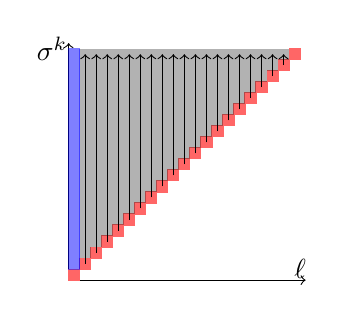
\begin{tikzpicture}[scale=0.14, shorten >=2pt]
            \draw (0,0) edge[->] (22,0);
            \draw (0,0) edge[->] (0,22);
            \node at (21,1) {$\ell$};
            \node at (-1.5,21) {$\sigma^k$};
            \foreach \i in {0,...,20} \draw[fill,red!60] (\i,\i) rectangle (\i+1,\i+1);
            \foreach \i in {0}{
               \draw[fill,blue,opacity=0.5] (\i,\i+1) rectangle (\i+1,21);
               \foreach \j in {1,...,19}{
                   \fill[black,opacity=0.3] (\i+\j,\i+\j+1) rectangle (\i+\j+1,\i+21);
               }
            }
            \foreach \i in {1,...,19}{
                \draw (\i+0.5,\i+0.5) edge[->] (\i+0.5,21);
            }
        \end{tikzpicture}
        &
        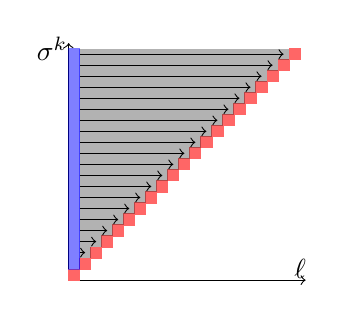
\begin{tikzpicture}[scale=0.14, shorten >=2pt]
            \draw (0,0) edge[->] (22,0);
            \draw (0,0) edge[->] (0,22);
            \node at (21,1) {$\ell$};
            \node at (-1.5,21) {$\sigma^k$};
            \foreach \i in {0,...,20} \draw[fill,red!60] (\i,\i) rectangle (\i+1,\i+1);
            \foreach \i in {0}{
               \draw[fill,blue,opacity=0.5] (\i,\i+1) rectangle (\i+1,21);
               \foreach \j in {1,...,19}{
                   \fill[black,opacity=0.3] (\i+\j,\i+\j+1) rectangle (\i+\j+1,\i+21);
               }
            }
            \foreach \i in {2,...,20}{
                \draw (1,\i+0.5) edge[->] (\i,\i+0.5);
            }
        \end{tikzpicture}
        &
        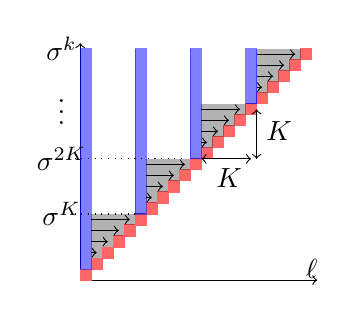
\begin{tikzpicture}[scale=0.14, shorten >=2pt]
            \draw (0,0) edge[->] (22,0);
            \draw (0,0) edge[->] (0,22);
            \node at (21,1) {$\ell$};
            \node at (-1.7,21) {$\sigma^k$};
            \foreach \i in {0,...,20} \draw[fill,red!60] (\i,\i) rectangle (\i+1,\i+1);
            \foreach \i in {0,5,10,15}{
               \draw[fill,blue,opacity=0.5] (\i,\i+1) rectangle (\i+1,21);
               \foreach \j in {1,...,5}{
                   \fill[black,opacity=0.3] (\i+\j,\i+\j+1) rectangle (\i+\j+1,\i+6);
                }
                \foreach \j in {2,...,5}{
                    \draw (\i+1,\i+\j+0.5) edge[->] (\i+\j,\i+\j+0.5);
                }
            }
            \draw (11,11) edge[<->] node[below] {$K$} (16,11);
            \draw (16,11) edge[<->] node[right] {$K$} (16,16);
            \node at (-1.7,6) {$\sigma^K$}; \draw[dotted] (-.5,6) -- (5.5,6);
            \node at (-1.7,11) {$\sigma^{2K}$}; \draw[dotted] (-.5,11) -- (10,11);
            \node at (-1.7,16) {$\vdots$};
        \end{tikzpicture} \\
        (a) \cite{akbarzadeh2020conditions,nino2020fast} use \eqref{eq:15}.
        &(b) Subroutine~\ref{algo:update_X}.
        &(c) Subroutine~\ref{algo:FMM}.
    \end{tabular}
    \caption{Comparison of the computation load of \eqref{eq:15} used in \cite{akbarzadeh2020conditions,nino2020fast} with the one of Subroutine~\ref{algo:update_X} and Subroutine~\ref{algo:FMM}. }
    \label{fig:apx_fast_mm}
\end{figure}

This  leads to the next fundamental  question: {why should the computation of Whittle index be harder than matrix inversion (or multiplication)?} To us, the main difference is that when computing Whittle indices, the permutation $\sigma$ is not known a priori but discovered as the algorithm progresses: $\sigma^k$ is only known at iteration $k$. Hence, while all terms of the matrices $X^k_{ij}$ are not needed, it is difficult to know a priori which ones are needed and which ones are not. Hence, a simple divide and conquer algorithm cannot be used. This is why when recomputing $\mX^{k+1}$ in Subroutine~\ref{algo:FMM}, we recompute the whole matrix (the vertical blue line) and not just the part that  will be used to compute the gray zone: we do not know \emph{a priori} what part of $X^{k+1}_{ij}$ will be useful or not.

\endgroup

\chapter{Carbon footprint}
\label{chapter:blabla2}

\lipsum[11-12]

